\chapter{图像有损压缩实验结果}

\section{实验结果的定性分析}
\begin{figure}[htb]
    \centering
    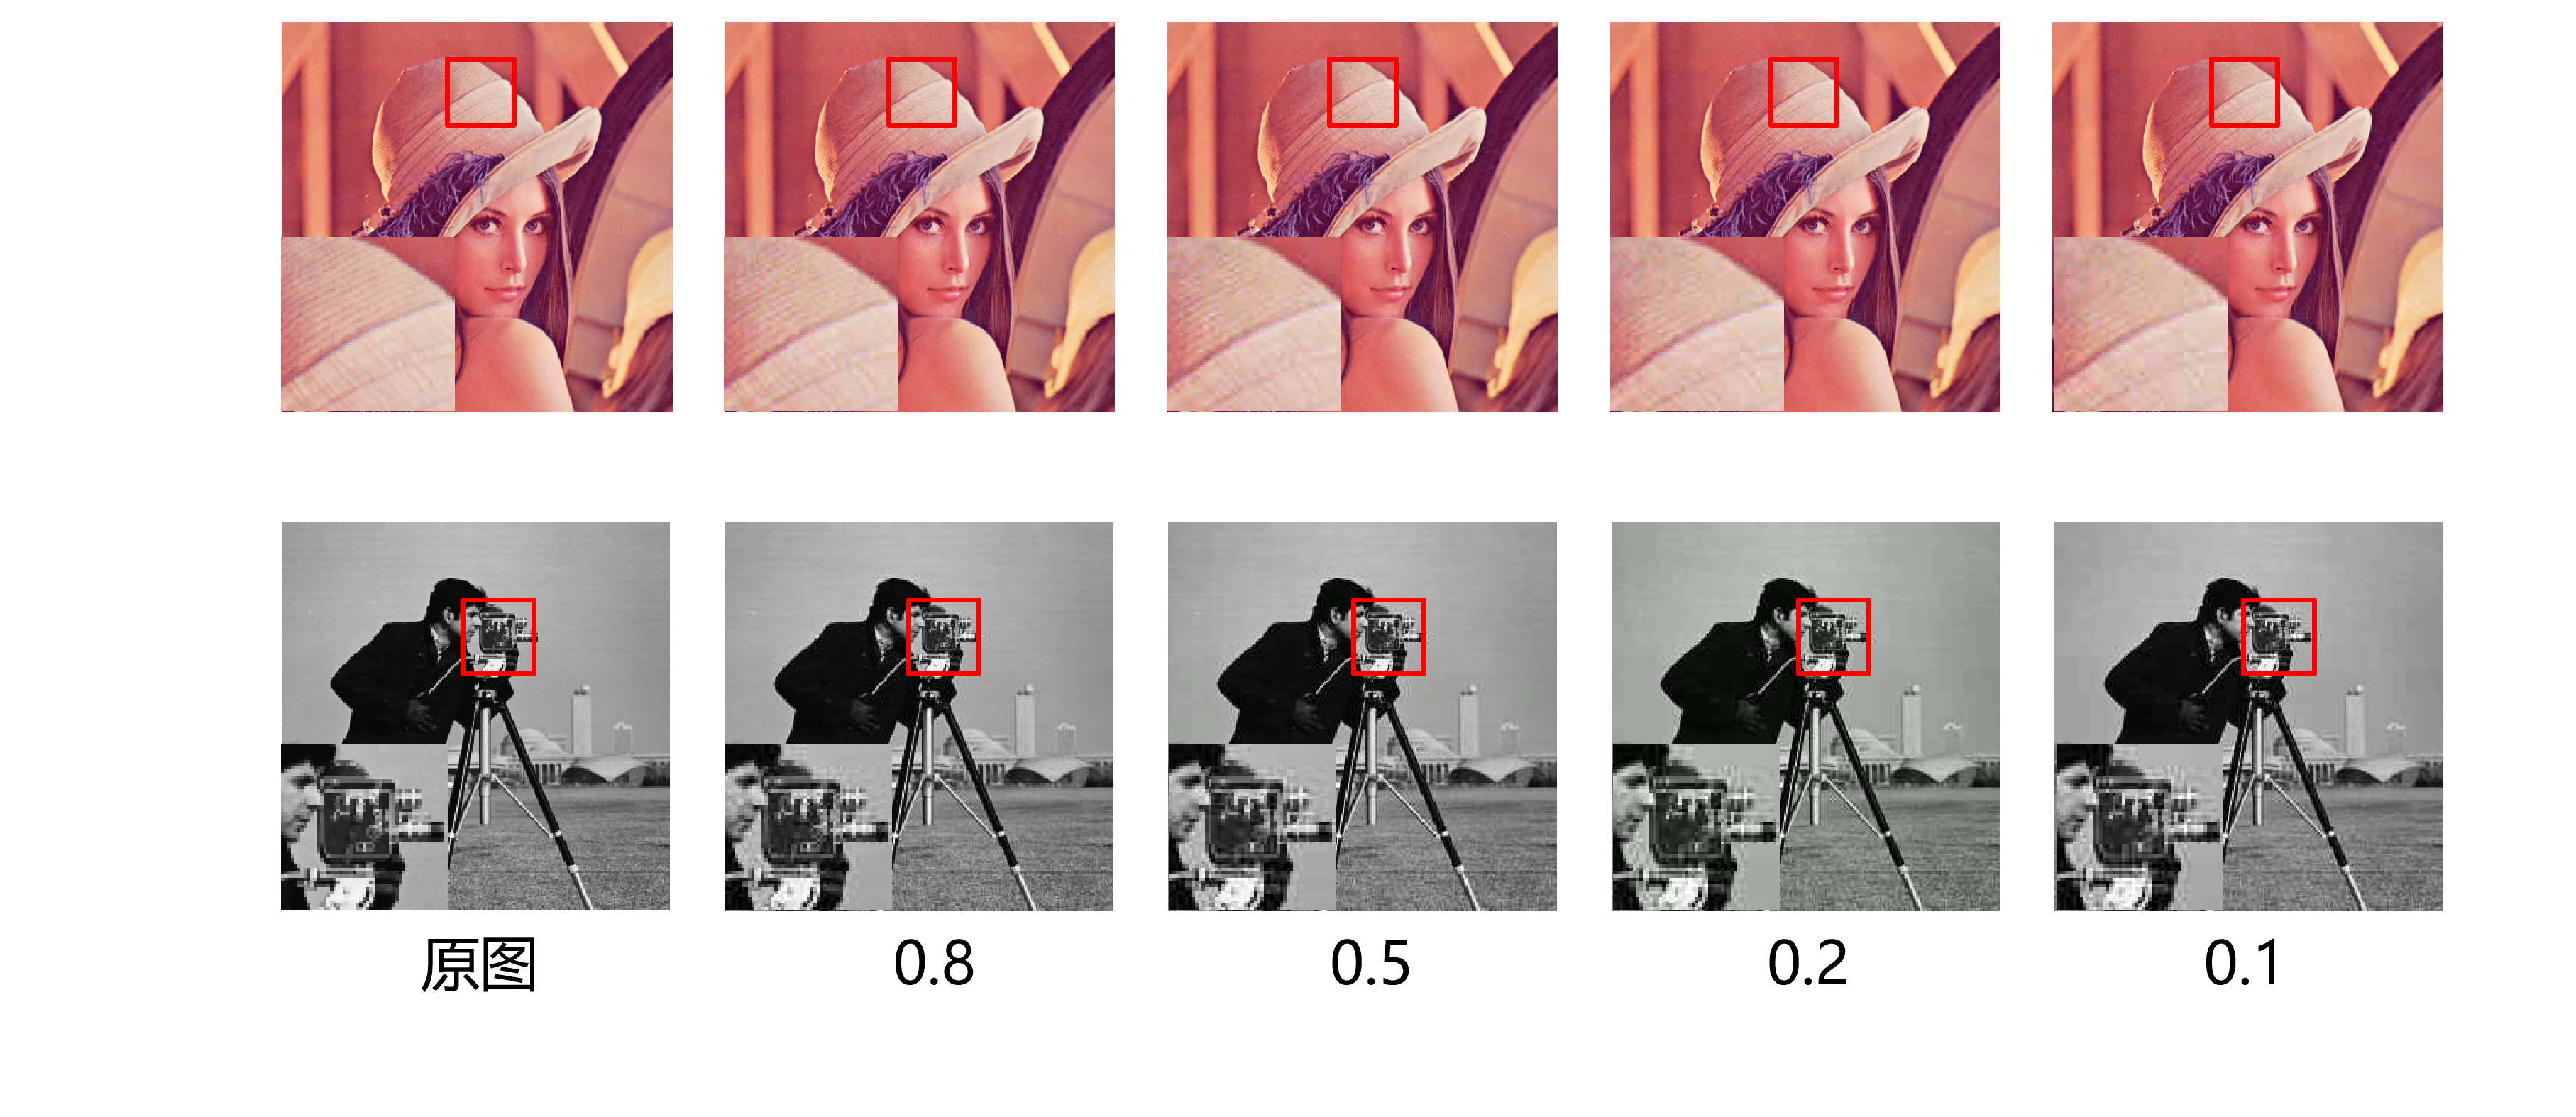
\includegraphics[width=1.0\textwidth]{pages/evaluation/result-image.png}
    \caption{实验结果的定性分析}
    \label{Fig.result}
\end{figure}

\section{实验结果的定量分析}
\subsection{性能指标}

\subsubsection{MSE}
均方误差(Mean-Square Error, MSE)是反映估计量与被估计量之间差异程度的一种度量。实验中定义为原图各像素$I(i,j)$与压缩后图像各像素$K(i,j)$差的平方和(式\ref{Eq.MSE})
\begin{equation}
    MSE=\frac{1}{mn} \sum_{i=0}^{m-1}\sum_{j=0}^{n-1} [I(i,j)-K(i,j)]^2
    \label{Eq.MSE}
\end{equation}
MSE值越小,代表压缩中损失的数据量越小。

\subsubsection{PSNR}
峰值信噪比(Peak Signal to Noise Ratio, PSNR)是一种评价图像的客观标准,它的单位是dB,用于衡量经过处理后的图像质量, $PSNR$ 值越大,就代表失真越少。图像的峰值信噪比定义为
\begin{equation}
    PSNR=20\lg (\frac{Max_1}{\sqrt{MSE}})
    \label{Eq.PSNR}
\end{equation}
其中$Max_1$是表示图像点颜色的最大数值,$MSE$是原图像与压缩图像之间均方误差(式\ref{Eq.MSE})。


\subsubsection{SSIM}
结构相似度(Structural Similarity Index,SSIM)是一种衡量两幅图像相似度的指标,在图像压缩中,用以衡量压缩前后的图像质量。原始图像$x$和压缩之后的图像$y$之间的结构相似度为
\begin{equation}
    SSIM(x,y)=\frac{2\mu_x\mu_y+C_1}{\mu_x^2+\mu_y^2+C_1}\cdot\frac{2\delta_{xy}+C_2}{\delta_x^2+\delta_y^2+C_2}
    \label{Eq.SSIM}
\end{equation}
其中$\mu_x,\mu_y$分别代表原始图像和恢复图像的均值,$\delta_x^2,\delta_y^2$分别代表原始图像和恢复图像的方差,$\delta_{xy}$是两图的协方差。$C_1,C_2$是维持稳定的常数,它们与像素值的动态范围有关。SSIM值越接近1,代表压缩后的图像结构与原始图像越接近,也即压缩中损失的数据越少,压缩质量越高。


\subsubsection{压缩比}
压缩比定义为原图片比特数与压缩编码后所占比特数之比。

\subsection{定量结果}

\begin{table}[h!]
    \begin{center}
        \caption{MSE}
        \begin{tabular}{c|ccccc}
            \textbf{压缩质量} & 0.8 & 0.5 & 0.3 & 0.2 & 0.1 \\
            \hline
            \textbf{MSE} & 4.92 & 5.40 & 5.73 & 5.90 & 6.00 \\
        \end{tabular}
    \end{center}
\end{table}


\begin{table}[h!]
    \begin{center}
        \caption{PSNR}
        \begin{tabular}{c|ccccc}
            \textbf{压缩质量} & 0.8 & 0.5 & 0.3 & 0.2 & 0.1 \\
            \hline
            \textbf{PSNR} & 41.2 & 40.8 & 40.5 & 40.4 & 40.3 \\
        \end{tabular}
    \end{center}
\end{table}

\begin{table}[h!]
    \begin{center}
        \caption{SSIM}
        \begin{tabular}{c|ccccc}
            \textbf{压缩质量} & 0.8 & 0.5 & 0.3 & 0.2 & 0.1 \\
            \hline
            \textbf{SSIM} & 0.9855 & 0.9838 & 0.9828 & 0.9822 & 0.9817 \\
        \end{tabular}
    \end{center}
\end{table}

\begin{table}[h!]
    \begin{center}
        \caption{压缩比}
        \begin{tabular}{c|ccccc}
            \textbf{压缩质量} & 0.8 & 0.5 & 0.3 & 0.2 & 0.1 \\
            \hline
            \textbf{游程压缩比}     & 7.99 & 9.88 & 10.9 & 11.4 & 11.8 \\
            \textbf{总压缩比}       & 13.0 & 16.2 & 18.2 & 19.2 & 20.0 \\
            \textbf{Matlab压缩比}   & 17.8 & 32.3 & 44.5 & 56.6 & 82.2 \\
        \end{tabular}
    \end{center}
\end{table}

定量实验结果如上表所示,其中游程压缩比为游程编码结束后对(值,串长)所占空间进行计算所得出的压缩比,总压缩比为哈夫曼编码结束后对二进制比特流和编码表所占空间进行统计所得出的压缩比,也是本次仿真实验得出的压缩比。Matlab压缩比为使用Matlab自带函数imwrite进行JPEG压缩所得到的压缩比。

可见,压缩质量系数越低,均方误差MSE越大,峰值信噪比PSNR越小,结构相似度SSIM越低,压缩比越大,符合预期。仅分析压缩比可以看出,游程编码后已经可以得到10左右的压缩比,冗余信息已经在一定程度上被压缩。哈夫曼编码能把游程编码的结果进行进一步压缩,获得更高的压缩比,这是因为游程编码属于统计编码,基于数据的重复特性来编码以达到减少数据量的目的,而哈夫曼编码是一种熵编码,从信息论的角度应用变长编码追求数据的压缩。它们从不同的角度进行数据压缩,故可以叠加使用。

对比Matlab自带函数实现的JPEG压缩,我们的仿真实验还存在一些不足,比如游程编码时我们对YUV三个通道分别进行,没有将所有数据统一到一起;霍夫曼编码时没有采用官方推荐的编码表;对连0的情况没有进行特殊处理。这些仿真实验与真实算法的差异导致了我们的压缩比距离理想值还有差距。
